\expandafter\ifx\csname ifdraft\endcsname\relax
\documentclass[11pt]{jsreport}
\usepackage{mypackage}
\begin{document}
\fi

\chapter{情報伝達経路モデルに基づく対話的不具合分析手法の仕様}

\section{概要}
本研究では,衛星の不具合分析において故障仮説の検証を支援するシステムを提案する.

%目的に書いていたところをここに持ってきてその要素に関して詳細に述べる.
以上の機能を満たすために,本手法は下記の3つの要素で構成されている.
\begin{itemize}
   \item 衛星内部機器の接続関係モデル及び,情報伝達経路モデル
   \item 故障箇所の特定を行うために必要なコマンド及びテレメトリの探索アルゴリズム %ここの言い回し
   \item コマンドの安全性,及び故障候補切り分け能力を示す指標
\end{itemize}


%具体的にどのような支援を目指すのか?
具体的には,本手法はコマンドとテレメトリをベースにして行う不具合分析を対象にしており,
不具合発生時に故障箇所を特定するために,確認すべきテレメトリ,打つべきコマンド
を選択肢として提示することで,人間が実機に対して打つコマンドを選択する際の
判断の支援を行う.\\
%ここに自分の意志が入っているのはおかしい?
また,不具合原因特定の全ての過程を衛星の制約モデルを用いて行うためには,%制約モデル?
非常に忠実度の高いモデルが必要である.衛星は複雑に物理現象が絡み合う
ため,物理法則に基づいた事象が各コンポーネント間を伝搬する様子を表現することは
モデル化のコストが非常に大きい.
むしろ,人間を対話的に支援することによってモデルに求められる忠実度のレベル
を下げつつ不具合分析の過程を体系化することができ,経験の少ないエンジニアの支援が
できる.そのため,システムが提示した選択肢を用いて人間が実機での検証を行い,
その検証結果をシステムに反映することで,対話的に故障箇所の特定を行っていく
構成となっている.\\
%ここに手法の簡単な構成を入れたほうがいいのか?提案手法の中にまとめてしまうのか?



%最終的に目標とするシステムの流れを示す.これはアルゴリズムではなく,概要
以下の図\ref{fig:fault_diagnosis}に,本手法を用いて不具合分析を行う流れを示す.
本研究の対象は,図\ref{fig:fault_diagnosis}で色付けしているところであり,
不具合発生時の異常テレメトリ情報が与えられてから,故障仮説の生成,
その仮説を検証するための「コマンド及び確認事項」を探索し,人間に提案を行うところまでである.

%検証結果のフィードバックもできるようにする予定.
%ただし,OK NGという簡単なフィードバック.パラメータ的な状態量は組み込めていない
\begin{figure}[H]
   \centering
      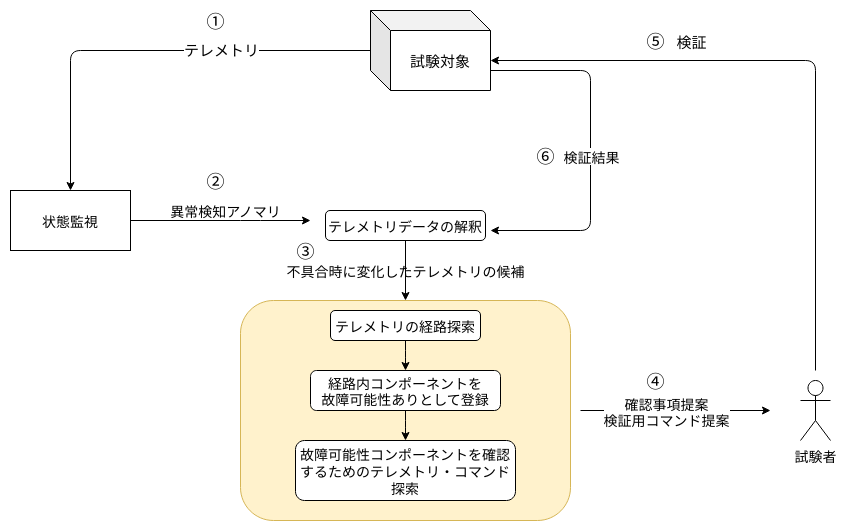
\includegraphics[height=9.0cm]{figure/fault_diagnosis_flow.png}
      \caption{不具合分析の流れ}
      \label{fig:fault_diagnosis}
\end{figure}

%図を修正して,それに対応してこれも修正する.
本手法を用いた不具合分析の流れは以下である.
\begin{enumerate}[1]
   \item 異常検知のきっかけとなったテレメトリ群を与える.
%   どこが異常値なのかを認識させる. 
   %不具合を起こしたトリガーが何なのかは分からないが,コマンドによってもたらされたかの区別だけ必要?
   \item 1で得たテレメトリに影響を与えるコマンドを送信されてから,
   地上局がテレメトリを受信するまでの一連の経路を取得する.
   \item 得られた経路内にあるコンポーネントを「故障候補」として登録する(故障仮説の生成).
   %その経路に対してコマンドパスとして入力があれば,入力の元となっているコンポーネントも故障候補に追加する.
   %ココらへんの細かい流れは図に表現できていないので,あとで説明する形を取る
   %\item 他のテレメトリを確認することによって,棄却できる「故障候補」を棄却する.
   %\item コマンドを送って得られるテレメトリ情報によって,故障候補を確認することができるコマンドの探索を行う.
   \item 打つコマンドが無くなるか,不具合原因の特定ができるまで以下を繰り返す.
   \begin{enumerate}[\textrm{4.}1]
      \item 故障候補を確認するためのテレメトリ及びコマンド探索
      \item 上で得られたコマンド及び確認事項を,人間の判断を支援する指標と共に
      提示する.
      \item システムが提示した情報を元に人が打つコマンドを選択し,仮説の検証を行う.
      \item 送信コマンドに対するテレメトリを確認し正常かどうかのフィードバックを行う.
      \item 人間からのフィードバックに応じて故障仮説の棄却及び,モデルが持つ状態の更新を行う.
   \end{enumerate}
\end{enumerate}
%
故障候補を確認するためのテレメトリ・コマンド探索の流れの詳細に関しては
後ほど言及する.

%また,本手法では故障候補は異常テレメトリが通る経路内にあるコンポーネントとしており,
%網羅的に洗い出せているとは言えない.

%実践した結果を分かりやすく表示させるように変更して,
%その結果を例に説明するのがいいかもしれない
\subsection{故障候補を切り分けるためのコマンド及び確認事項の探索}
以上で述べた不具合分析アルゴリズムにおける,
故障候補の中から切り分けを行うためのコマンド,及び
確認事項の探索に関して,本手法における仮定とともに詳細を述べる.\\
不具合が発生している状態で予期せぬ二次故障を起こさないために,
探索順序としては,衛星の状態を変えずに確認できるものを優先的に探索
することが望ましい.
%ここ表現がわかりにくい
そのため,不具合発生時に取得しているテレメトリの中から
不具合原因特定に役に立つテレメトリ情報が存在するのであれば,
そのテレメトリを確認事項として提案する.\\
その後,衛星の状態を変化させること無く
故障原因特定のために得られる情報がなくなれば,
次ステップとしてコマンドを打って得られる
情報から切り分けを行っていくことになる.
このとき,残ったコマンドで故障候補の状態を確認できるものを探索し,
上で示した指標の計算を行い提示する.
%提示するコマンド候補としては,使用するコンテキストに適した評価指標に基づいて
%上位 のコマンドを指標の値とともに提示する.
%ここにフローチャート的なものあるといいよね




%ここにモデルの説明
%これらのモデルに基づいて,実装上ではどのようなオブジェクトが生成され
%どのように関係しているのかを図示できたほうがいい
\section{事前定義モデル}
次に,以上で述べたアルゴリズムで不具合分析を行うために必要なモデル
に関して,具体的なテストケースをベースにして説明する.%言い回し

%これも既にモデル.先にどんなモデルが必要になるのかをまとめておいたほうがいいのか?
\subsection{対象とするテストケース}
今回,以下の図\ref{fig:simple_sat}の
ような簡易衛星モデルを対象にしてモデルの定義及び
不具合分析手法の実践を行う.\\
また,矢印の色が情報の方向性を表しており,赤がコマンドによる情報の伝達,
青がテレメトリによる情報の伝達である.また,矢印の種類が情報として伝わる物
を表しており,それぞれ以下のようになっている.
\begin{itemize}
   \item Signal:電気信号
   \item Power:電源
   \item Heat:熱
\end{itemize}
\begin{figure}[H]
   \centering
      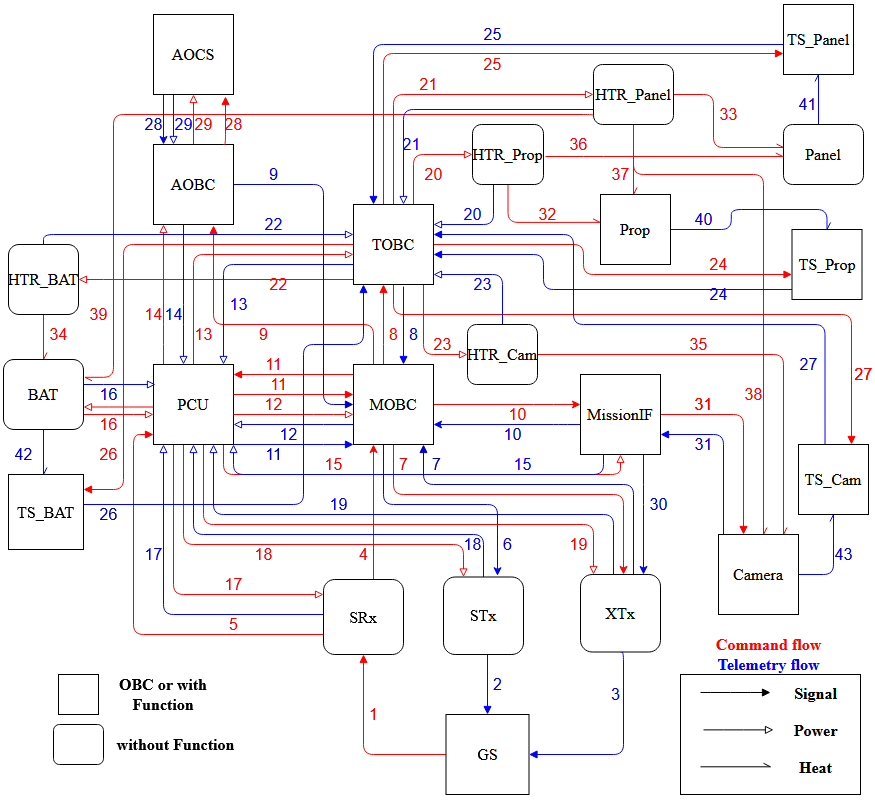
\includegraphics[height=13.0cm]{figure/satellite_diagram.png}
      \caption{簡易衛星モデル}
      \label{fig:simple_sat}
\end{figure}

\subsection{各コンポーネント間の接続関係モデル}
來村ら\cite{Kitamura01}は拡張デバイスオントロジーとして,
機器を構成する装置間のつながりを表現するために「ポート」と「導管」%ここの説明を考える
という概念を定義している.このオントロジーを用いて,山口ら\cite{Yamaguchi2014}
は人工衛星デバイスオントロジーを構築している.
%論文ではもう少し詳細に説明する.
これらを参考にし,以下の表\ref{tab:link_definition}のように
接続関係を「リンク」として定義した.\\%違いを説明する必要があると思う
リンクが持つ情報としては,リンク名,接続コンポーネント,ID,伝達物,
そのリンクが正常に情報伝達を行う確率%言葉がむずい
となっており,IDが各リンク固有の識別子としてリンクを参照する際に
使用される.また,実際にコンポーネント間を接続している実態(配線やコネクタなど)を表現している
のではなく,接続関係を概念的に表現したものにすぎない.
%そのメリットは何なん?
%ほんまはちゃんとポートと導管を作ったほうが良かったんかもしれん

%\newpage
%キャプションとくっついているか確認
%図新しいのに変える
\begin{table}[H]
   \centering
   \caption{リンク定義例}
   \label{tab:link_definition}
\end{table} 
\vspace{-2zh}
\begin{figure}[H]
   \centering
      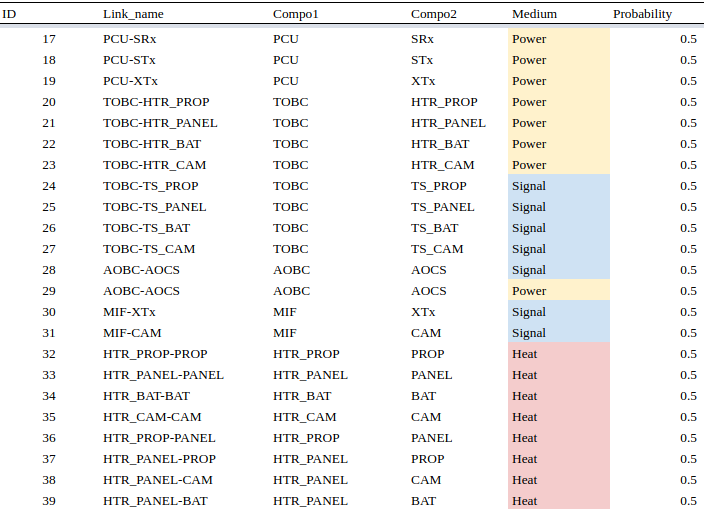
\includegraphics[height=11cm]{figure/link_definition.png}
\end{figure}

次に,コンポーネントの定義を行う.以下の表\ref{tab:compo_link}では,
衛星システム全体で使用されている
コンポーネントのリストを作成し,各コンポーネントが接続している
コマンドリンクとテレメトリリンクを,上で定義したリンクのID
を用いて定義している.
ここで,コマンドリンクというのはコマンドによる情報の伝達で使用されるリンクであり,
テレメトリリンクというのはテレメトリによる情報の伝達で使用されるリンクである.
この時,コンポーネントが属性として持つリンクはそのコンポーネントが出力元となる場合としている.

%キャプションとくっついているか確認
%図新しいのに変える
\newpage
\begin{table}[H]
   \centering
   \caption{コンポーネント定義例}
   \label{tab:compo_link}
\end{table}
\vspace{-2zh}
\begin{figure}[H]
   \centering
      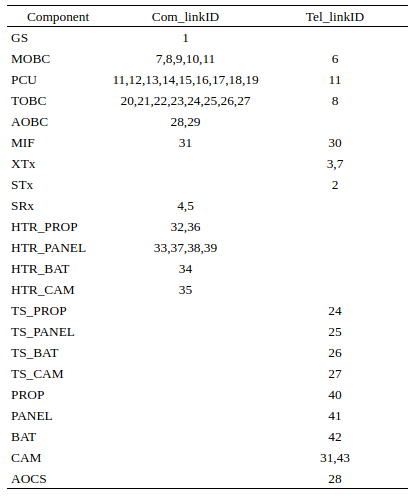
\includegraphics[width=10cm]{figure/compo_link.png}
\end{figure}

以上の情報によって,衛星内部でコンポーネント全体がどのように接続しているか
を定義することが可能になる.\\
%なんか説明が微妙
また,各コンポーネントの状態を以下の
図\ref{fig:Compo_state}のように定義する.
本研究では,簡単のため扱う状態は,各コンポーネントの電源状態,
それに伴う電力消費,姿勢変化及び,熱の発生としている.
また,電源ON/OFF状態以外にも機能を持つコンポーネントは
その機能をFunctionで定義しており,機能の
動作状態がコマンドによって操作される構成となっている.
初期状態を図\ref{fig:Compo_state}のようなファイル形式で与え,
その後の状態の更新は人間が選択したコマンドが持つ機能情報に基づいて
行うようにしている.
%現状のモデルではON/OFF状態や機能動作の正否のような2値状態のみしか扱えていないが,
%将来的にはパラメータを含む状態量も扱えるように拡張していく予定である.
\begin{figure}[H]
   \centering
      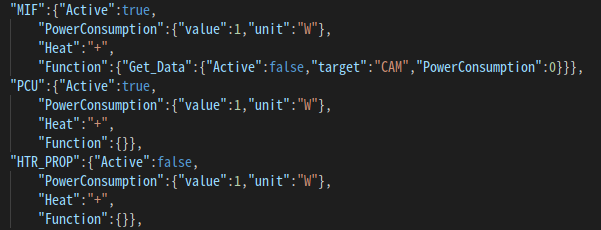
\includegraphics[height=5.0cm]{figure/Component_state.png}
      \caption{コンポーネント初期状態例}
      \label{fig:Compo_state}
\end{figure}

\subsection{コマンド・テレメトリの情報がコンポーネント間を伝わる経路のモデル}
今回の衛星モデルにおけるテレメトリ及びコマンド
を以下の表\ref{tab:telemetry},\ref{tab:command}に定義した.\\
まず,本手法で用いるテレメトリの情報は,ID,テレメトリの名前,
テレメトリが変化するためのトリガー,テレメトリの情報が衛星内部及び地上局まで伝わる
経路である.%利用可かどうかは?
今回は簡単のため,状態が変化するためのトリガー(TransitionTrigger)として,
時間とコマンドのみを考えており,姿勢変化や軌道条件に依存した
状態変化は考えないことにする.また,経路は通るリンクのIDを用いて
表現している.
時間変化するテレメトリに関しては,コマンドによって状態変化をさせなくても
変化を確認することが可能なので,不具合分析の初めのアプローチに利用可能である.

%経路はjsonで記述したほうが扱いやすいし,分かりやすい.時間あれば実装も含めて修正
%経路だけじゃなくて,遷移するトリガーも加えたことを記述
%テレメトリも種別必要なんじゃね?あと,降りているかどうかという状態も必要そう.
%ここに書くかは別として
\newpage
\begin{table}[H]
   \centering
   \caption{使用テレメトリ}
   \label{tab:telemetry}
\end{table}
\vspace{-2zh}
\begin{figure}[H]
   \centering
      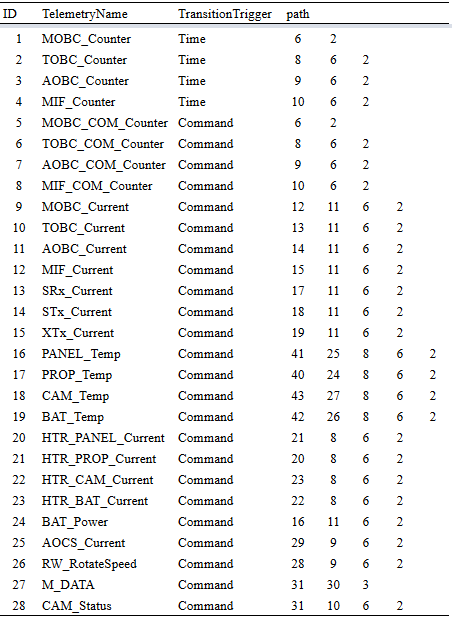
\includegraphics[width=10.0cm]{figure/TEL.png}
\end{figure}

また,コマンドの情報としてID,コマンドの名前,コマンドによって影響を受ける
テレメトリのID,コマンドの種別,コマンドによって情報が伝達する経路を与えている.
今回,表\ref{tab:telemetry}に示すテレメトリの経路及び,表\ref{tab:command}
に示す経路と影響テレメトリIDに関しては事前に定義したものを使用した.

また,コマンドが持つ機能によって,いくつかの種別に分類することができる.
JAXA\cite{JAXA2020}は,衛星と衛星搭載機器の機能をモデル化し,機能情報の
再利用性を高めることを目的とした手法を提案している.
今回,その手法の中の一部を採用しコマンドの種別を2種類(ACTION, GET)定義した.
また,各コマンドが持つ機能に関する情報を
以下の図\ref{fig:COM_type}のように定義している.
これによって,各コマンドが
上記で定義したコンポーネントが持つ機能を操作するという関係性を表現可能になる.
%この情報を用いて,不具合原因特定のためのコマンド
%を探索する際に有効となるコマンドを判断している.

\newpage
\begin{table}[H]
   \centering
   \caption{使用コマンド}
   \label{tab:command}
\end{table}
\vspace{-2zh}
\begin{figure}[H]
   \centering
      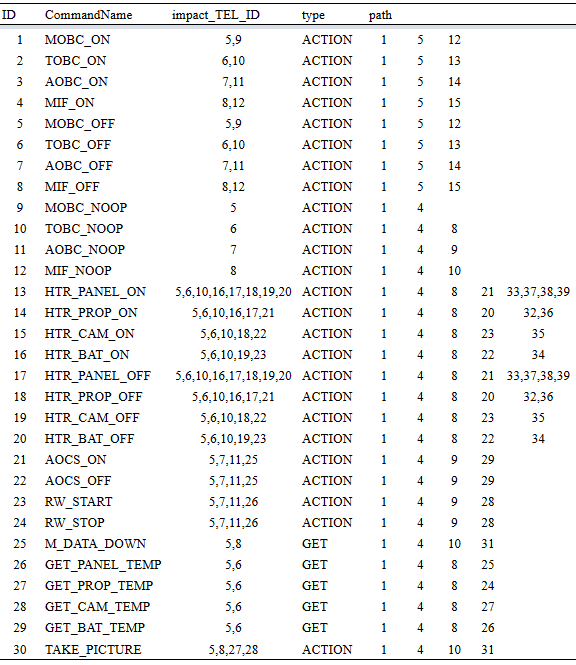
\includegraphics[width=13cm]{figure/COM.png}
\end{figure}

\begin{figure}[H]
   \centering
      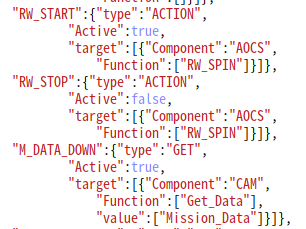
\includegraphics[height=5.0cm]{figure/COM_type.png}
      \caption{コマンドの機能モデル}
      \label{fig:COM_type}
\end{figure}


\section{探索アルゴリズム}
故障候補を確認するためのコマンド及びテレメトリをどのように探索するのかについての説明
フローチャートを用いたアルゴリズムの説明.



\section{コマンド評価指標}
次に,上記のアルゴリズムによって故障候補の切り分けを行う際,
人間がコマンドを選択するための指標に関して説明する.
%ここに軽く指標に関してどのような指標が必要なのか書いたほうがいいかも
不具合分析を行う際,衛星の安全を確保しながら正確な故障箇所の特定を行うことが,
地上での不具合改修に必要である.
そのため,コマンドが衛星にとって安全であることが重要である.\\
また,本研究の当初の目的は地上試験における不具合分析支援であったが,提案手法は
コマンドとテレメトリの粒度で得られる情報を用いて不具合分析を行っているため,
軌道上での運用時にも活用できると考えられる.
運用時には地上試験時とは異なり,不具合改修のための時間制約が発生することがあるため,
地上試験時とは異なる指標が必要となる.
そのため以下では,地上試験時と運用時の両方に関してコマンドを選択する上で必要な指標として
コマンドによる衛星生存性への副作用を示す指標とコマンドの故障候補の切り分け能力を示す指標
を提案し,
システムの使用状況に合わせてそれらの評価指標を切り替えることのできる
フレームワークであることを示す.

%確認することに関してはここで述べているのでこの仮定を置いていることに関してはここでいえばいいかもしれない
また本手法では簡単のため,コマンド及びテレメトリが情報を伝達する経路内に
故障候補が存在していれば,その故障候補を「確認できる可能性がある」としている.
一方で,各コンポーネントの状態を一切変えないコマンドや,コマンドを送っても
テレメトリに変化として現れない組み合わせは,不具合原因特定のために得られる情報がないため
「確認できる可能性がない」としている.\\
ここであくまでも「確認できる可能性」として記述しているのは,
情報が通る経路に故障候補が含まれていたとしても,伝達の
途中で情報が途切れてしまえば,その故障候補の状態を
確認することはできないためである.

\subsection{コマンドによる衛星生存性への副作用}
打つコマンドが安全であるかという点は,衛星の状態に依存するが,不具合発生時には
衛星の状態把握が十分に行えていない状況であるため,
網羅的にリスクを考慮した安全性を評価するのは困難である.
そこで,以下では簡単に電力と姿勢の制約を元に,コマンドの危険性を定量化する
ための指標を示す.

%BAT残量の定義がおかしいことに関して,どのような仮定をおいているのかを説明するべき
まず,運用時には発電量と各コンポーネントの電力消費状態に応じて
電力の制約が発生する.バッテリ残量が少ない状態で大きな電力を消費するコンポーネントの
電源をONにするといった行為は,衛星が生存するために必要な機能を動作させるための
電力を枯渇させる可能性があるため,危険な行為であると言える.
そのため,故障箇所の特定を行うためにコマンドを打つ際には,現在の衛星の電力状態を
把握し,コマンドを打つことで電力不足にならないかを確認しながら行動を起こさなければならない.
%もう一文くらいあってもいいかもね
コマンドを選択する際に電力に関する制約を明示的に示すことは,未熟なエンジニアが
誤ったコマンドを打つことを防ぐために効果的であると考えられる.
そのため本手法では,コマンドの副作用を示す一つの指標として「バッテリ残量」
と「コマンドを打つことによって発生する消費電力」を示すことにする.
ここでは電力による制約を簡単に表現するため,
バッテリ残量は電源がONになっている機器の消費電力のみから計算することとし,
姿勢の変化や日照条件に応じた充電量の変化は考慮していない.

次に,姿勢の制約による指標に関して述べる.
軌道上で姿勢が変化すると日照条件や入放熱量など,様々な波及効果が考えられ,
衛星の状態が大きく変化する.一方で,上で述べたように不具合発生時には
衛星の状態に不確定な要素が多く含まれているため,意図せず姿勢変化を起こし
状態を大きく変化させることは非常に危険である.
本手法で用いるモデルでは姿勢が変化することによる各状態量への影響は考慮していないが,
将来的に実ミッションで使用することを考えると,%???
姿勢変化は衛星の生存にとって
リスクの大きな動作であるとため,「姿勢変化を起こすか否か」を二つ目の指標として
提示する.

最後に,コマンドによる波及効果の大きさを示す指標に関して述べる.
上述したように,状態を大きく変化させるようなコマンドを故障個所の特定
のために用いることは望ましくない.
そこで,コマンドによって発生する衛星内部状態の変化の大きさを
%簡単にはテレメトリの数でいい気がするが..とりあえず保留
%上記で定義したコンポーネントの状態(電源状態及び機能動作状態)
%が変化した数を用いることにする.
「コマンドを打つことで変化する
テレメトリの数」を用いて定量的に示す.
これは,事前にコマンドの定義によって定められている
「コマンドに影響を受けるテレメトリ」と,人間からフィードバックを受けながら更新される
衛星内部コンポーネントの状態から求めることが可能である.この情報を示すことで,
コマンドが引き起こす衛星内部の状態変化の大きさを
人間に対して認識させることが可能である.\\
以上で述べたコマンドの副作用を示す3つの指標を以下に再掲する.
\begin{itemize}
   \item コマンドを打つ前のバッテリ残量と,コマンドを打つことによって発生する消費電力
   \item 姿勢変化を起こすか否か
   \item コマンドを打つことで変化するテレメトリの数
\end{itemize}

%初めに切り分け能力として,確認可能性と総コマンド数の2点に関して述べることを言ったほうがいい
\subsection{コマンドの故障候補切り分け能力}
%可視時間でもいいのか?
運用時には,通信可能な時間(以下,可視時間)が限られており,その時間中に不具合原因を特定
しなければならないような時間制約がある場面が存在する.
運用形態によっては,可視時間が非可視時間に比べて非常に短いこともあり,
その際には一つの可視時間を逃すとミッション失敗につながるため,%言い方
少ないコマンド数で効率的に不具合分析が行えることが重要である.\\
以下では,一つのコマンドの故障候補切り分け能力を表す指標と,
ある故障候補がある際にどのコマンドから検証を始めれば最終的に少ないコマンド
数で終えることができるかを表す指標の2点に関して述べる.

\subsubsection{コマンドが確認できるリンクの数}
効率的な不具合分析を行うためには,一度に確認できる故障候補の数が多いことが望ましい.
コマンドによる検証を行う際,検証結果が正常テレメトリであれば,そのコマンドとテレメトリで形成される
経路内にある故障候補は正常であると言えるため,故障候補の切り分けを行うことができる.
一方で,選択したコマンドによる検証結果が異常テレメトリであった場合,
伝達する情報が経路内のどこで異常になったかが分からなければ,その経路内に
存在する故障候補の切り分けを行うことはできない.
そのため,経路内に多くの故障候補が存在する場合でも,
切り分けの能力が高いとは言えない.故障候補の切り分け能力を考えるためには,
検証結果が正常,異常に関係なく経路内にある
故障候補をどれだけ確認できるかが重要になる.
以下では,故障候補にあるリンクが正常に情報を伝達できる確率を用いて,
コマンドが確認できるリンクの数を見積もる.
%あとここで言っている正常はつながりが切れていないかという点であることを説明する?
各コマンドによって情報が伝達し,テレメトリとして地上局に返ってくる経路によって,
確認する対象のリンクまでに通る経路が異なる.
その各経路に存在するコンポーネントをつなぐリンクが正常である確率を
$P(l = \text{normal})$,異常である確率を$P(l = \text{abnormal})$ %確率Pも斜体じゃないほうがええかも
として与える.
あるリンク$l_i$を確認するためには,リンク$l_i$が接続されているコンポーネントまでの経路
が正常であることが必要である.このことから,「リンク$l_i$を確認することができる確率」
がそれぞれの経路によって定まる.このことを以下の図\ref{fig:route}に示す例を用いて示す.
以下では簡単のため,$P(l_i = \text{normal}) = P(l_i = \text{abnormal}) = 0.5$であるとし,
太矢印になっている箇所が故障候補である.また故障候補以外は正常であるとし,
正常なリンクに関しては$P(l_i = \text{normal}) =1$である.\\
\begin{figure}[H]
   \centering
      \begin{tabular}{c}
         \begin{minipage}{0.30\hsize}
         \centering
         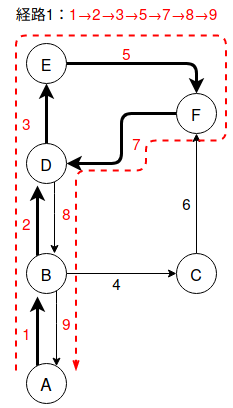
\includegraphics[height=7cm]{figure/route1.png}
          %  \caption{}
            \label{fig:route1}
         \end{minipage}
         \begin{minipage}{0.30\hsize}
         \centering
         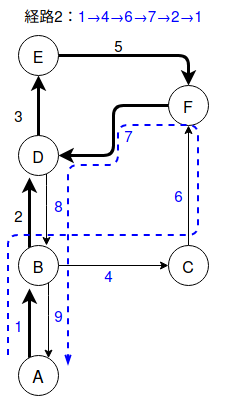
\includegraphics[height=7cm]{figure/route2.png}
         %\caption{}
            \label{fig:route2}
         \end{minipage}
         \begin{minipage}{0.30\hsize}
            \centering
            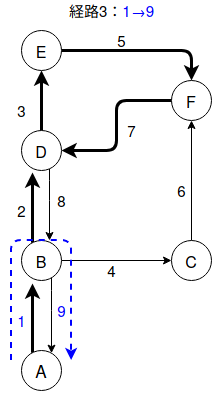
\includegraphics[height=7cm]{figure/route3.png}
            %\caption{}
               \label{fig:route2}
            \end{minipage}
      \end{tabular} 
      \caption{故障候補とそれを確認するための情報伝達経路の例}%ここも変えたほうがいいかも
      \label{fig:route}
\end{figure}
図\ref{fig:route}では,あるコマンドC$_1$によって影響を受けるテレメトリ
が3つ存在する場合を示している.
各テレメトリとコマンドC$_1$が形成する経路は異なり,それぞれ経路1,2,3としている.\\
この時,それぞれの経路に関して
リンク1を確認することができる確率を考えることにする.まず,経路1でリンク1の確認をするためには
ノードBからノードDまでの経路(2,3,5,7)
が正常である必要がある.%正常の定義を明確に
ここで,経路を表す記号をR,経路内にある故障候補リンクの集合を$\mathbb{F}$とすると,
経路1を通る情報でリンク$1$を確認することができる確率は

%これは同時確率でしかなくて,多分条件付確率ではない.というか同時確率でもない.Rjは事象ではない
\begin{eqnarray}
   P(l_{1} | \text{R}_1) &=& \prod_{i\in\mathbb{F}_1,i\neq 1} P(l_{i} = \text{normal})\\
     &=& \left( \frac{1}{2}\right)^4
\end{eqnarray}
であることが分かる.ここで,R$_1$は経路1,また
\begin{eqnarray}
   \mathbb{F}_1  &=& \{ 2,3,5,7\} 
\end{eqnarray}
である.\\
同様に経路2,3に関してもリンク$1$を確認することができる確率を求めると
\begin{eqnarray}
   P(l_{1} | \text{R}_2)  &=& \prod_{i\in\mathbb{F}_2,i\neq 1} P(l_{i} = \text{normal})\\
   &=& \frac{1}{2}\\
   P(l_{1} | \text{R}_3)  &=& \prod_{i\in\mathbb{F}_3,i\neq 1} P(l_{i} = \text{normal})\\
   &=& 1
\end{eqnarray}
となる.
このように,あるリンク$l_i$を通る経路が複数存在する場合,
経路に依存してそのリンク$l_i$を確認できる確率(以下では確認可能性とする)が変わる.
%なんで最大値を取るようにするのかの説明が必要になるかもしれない
ここで,あるコマンドC$_k$による情報伝達経路の中で,リンク$l_i$を通る経路
が複数存在する場合には,リンク$l_i$に対する確認可能性が最大となる
経路を用いて確認すればいいので,コマンドC$_k$による
リンク$l_i$の確認可能性はそれらうちの最大値を取るものとする.
コマンドC$_k$が影響を与える各テレメトリと成す経路の内,リンク$l_i$を含むものを
$\mathbb{R}_{ki} = \{ \text{R}_{1_i}, \cdots ,\text{R}_{N_{ki}} \}$(ただし$N_{ki}$は
リンク$l_i$を含む経路の数)とすると,
コマンドC$_k$によるリンク$l_i$の確認可能性は
\begin{eqnarray}
   P(l_i|\text{C}_k) &=& \max  \{ P(l_i|\text{R}_{1_i}), \cdots ,P(l_i|\text{R}_{N_{ki}}) \}
   \label{eq:P li Ck}
\end{eqnarray}
となる.\\
式(\ref{eq:P li Ck})は経路$\mathbb{R}_{ki}$内にある故障可能性リンク
全てに対して求めることができるので,
これらの平均を取り,そのコマンドの「平均確認可能性」と定義する.
平均確認可能性は,コマンドC$_k$が影響を与える各テレメトリと成す経路の集合を
$\mathbb{R}_{k} = \{ \text{R}_{1}, \cdots , \text{R}_{j},\cdots ,\text{R}_{N_{k}} \}$とし,
それぞれの経路内に存在する故障可能性リンクの数を$N_{F_{kj}}$,
集合$\mathbb{R}_{k}$全体で考えた時の数を$\mathbf{N_{F_k}}$とすると
\begin{eqnarray}
   P_m(\text{C}_k) &=& \frac{1}{\mathbf{N_{F_k}}}\sum_{i=1}^{\mathbf{N_{F_k}}}P(l_i|\text{C}_k)
\end{eqnarray} %記号何がええんやろ
と表すことができる.平均確認可能性は,コマンドとテレメトリが通る経路に含まれる
故障候補のうち,どれだけのリンクの状態を確認できるかという指標である.
つまり,この指標が高いほど経路内に存在する故障可能性リンクの多くを
確認できるということになる.%これいらんかも
%それ以下でもそれ以上でもないのか??

また,平均確認可能性を経路$\mathbb{R}_{k}$内にある故障可能性リンクの数$\mathbf{N_{F_k}}$
にかけると,コマンドC$_k$によって確認できるリンク数の期待値を求めることができ,
\begin{eqnarray}
   E(\text{C}_k) &=& \mathbf{N_{F_k}}P_m(\text{C}_k)\\
   &=& \sum_{i=1}^{\mathbf{N_{F_k}}}P(l_i|\text{C}_k)
\end{eqnarray} 
となる.これを「確認可能リンク数」と定義する.

ここで,図\ref{fig:route}に示すコマンド1に関して平均確認可能性及び,
確認可能リンク数を計算してみると
\begin{eqnarray}
   P_m(\text{C}_1) &=& \frac{1}{\mathbf{N_{F_1}}} \{P(l_{1} | \text{C}_1) + P(l_{2} | \text{C}_1) +P(l_{3} | \text{C}_1)
   +P(l_{5} | \text{C}_1) + P(l_{7} | \text{C}_1)\} \\
   &=& \frac{1}{5} \left\{ 1 + \frac{1}{2} + \left( \frac{1}{2}\right)^4 + \left( \frac{1}{2}\right)^4
    + \left( \frac{1}{2}\right)^4 \right\}\\
    &=& 0.3375 \\
   E(\text{C}_1)  &=& 1.6875
\end{eqnarray} 
となる.
結果からわかるように,通る経路に存在する故障候補の数
が必ずしも確認できるリンクの数に対応しているわけではない.
故障候補にあるリンクを通ることで不確定性が蓄積されるため,全体として経路内にある
リンクを確認できる確率は小さくなる.
平均確認可能性が高く,確認可能リンク数も高いものが
故障候補の切り分け能力が高いコマンドであると言える.

%本手法では簡単のために接続関係における故障のみを見ていると説明するべき
\subsubsection{故障箇所特定のためにかかるコマンドの総数}
次に,コマンドを選択する順番によって,故障箇所を特定するために打つコマンドの総数に変化が現れる
ことを示し,コマンドの総数の見積もりに関して述べる.
%単一故障だけを考えている.一つの故障を見つけた時点で終了するという過程での話.というより接続関係の話
まず,上で定義した各リンクに関する正常確率を用いることによって,各径路ごとの
平均確認可能性を以下の式(\ref{eq:P_R})のように求めることが可能になる.%名前を変えたほうがいいかも
これを「経路別確認可能性」と定義する.
\begin{eqnarray}
   P_m(\text{R}_j)  &=& \frac{1}{N_{F_{kj}}}\sum_{i=1}^{N_{F_{kj}}}P(l_i|\text{R}_j) \label{eq:P_R}
\end{eqnarray}
あるコマンドを送った際にテレメトリを確認するときは「経路別確認可能性」が高い順番に行うことで,
経路内にあるリンクの状態を確認し故障候補から棄却する,または故障箇所であると特定する可能性が高くなる
ため,効率的に絞り込むことが可能になる.
また,各テレメトリの検証結果に応じてそれ以降に確認するテレメトリによるリンクの確認可能性
が変化する.%この文言は必要ないかもね
つまり,各テレメトリの結果が正常である(もしくは異常である)確率は他のテレメトリの結果
に依存することになる.\\
まず簡単のため,他のテレメトリの結果を考慮せずにテレメトリが正常(または異常)となる確率
に関して述べる.
テレメトリの結果が正常であるためには,そのテレメトリが通る経路内の
リンクがすべて正常であればよいので,コマンドC$_k$を送った時に
テレメトリT$_j$が正常または異常である確率は以下の式(\ref{eq:P_TEL_normal}),(\ref{eq:P_TEL_abnormal})
のようになる.この時,経路の添え字とテレメトリのIDが対応している.
\begin{eqnarray}
   P(\text{T}_j = \text{normal}) &=& \prod_{i\in\mathbb{F}_j} P(l_i = \text{normal}) \label{eq:P_TEL_normal}\\
   P(\text{T}_j = \text{abnormal}) &=& 1 - P(\text{T}_j = \text{normal}) \label{eq:P_TEL_abnormal}
\end{eqnarray}

次に,上述したように「経路別確認可能性」が高い順でテレメトリを確認して行った場合に,
各テレメトリの結果に応じて以降のテレメトリの正常(または異常)確率がどのように変化していくのかを示す.
以下の図\ref{fig:TEL_result_process}では,上で示した例(図\ref{fig:route})
に関して各テレメトリの結果ごとに,それ以降の結果を場合分けしたものを示している.
この時,図\ref{fig:route}の例では確認可能性は経路3,2,1の順に高いため,
その順番に従って検証を行っている.
\begin{figure}[H]
   \centering
      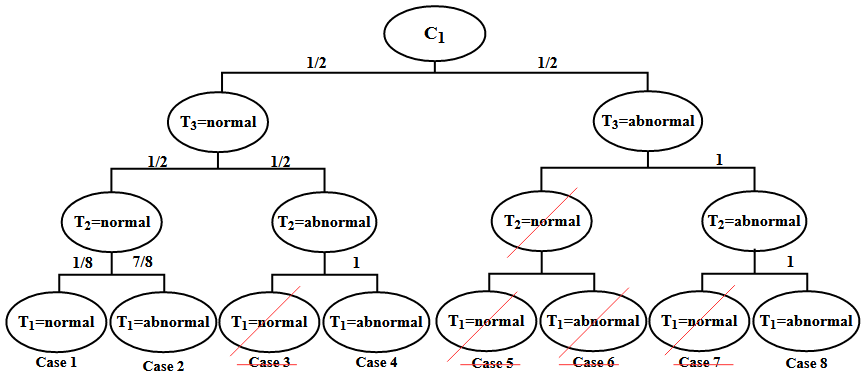
\includegraphics[height=6.0cm]{figure/TEL_result_process.png}
      \caption{各テレメトリの結果による検証過程の種類}
      \label{fig:TEL_result_process}
\end{figure}
まず,コマンド1を送信した際にテレメトリ3を確認すると,図\ref{fig:route}の経路3
が情報伝達経路であるため,その経路内に存在する故障候補はリンク1のみであり,
そのテレメトリの結果の確率は
\begin{eqnarray}
   P(\text{T}_3 = \text{normal})  &=& P(l_1 = \text{normal}) = \frac{1}{2} \label{eq:P_TEL3_normal} \\
   P(\text{T}_3 = \text{abnormal})  &=& P(l_1 = \text{abnormal}) = \frac{1}{2} \label{eq:P_TEL3_abnormal}
\end{eqnarray}
と求まる.これ以降の各テレメトリの結果の確率はT$_3$の結果に依存することになる.
まず,T$_3$が正常である場合を考えると,これによってリンク1は正常であることが確認できるため
リンク1は故障候補から除かれ,テレメトリ2の結果に関する確率は図\ref{fig:TEL_result_process}に示すように
求まる.同様に,テレメトリ1の結果に関する確率も,それ以前に確認した
テレメトリの結果によって経路内に存在する故障候補を更新した上で求めると図に示すようになる.\\
次に,T$_3$の結果が異常であった場合を考えると,経路3に含まれる故障候補はリンク1のみであるため,
リンク1の故障が確定する.
%ここの説明難しいな.言いたいのは故障箇所が一つでも含まれている経路を通るテレメトリは異常になるという
%仮定をしていること.
この時,以降に確認するテレメトリ2,1の結果は,T$_3$が正常である場合のときと同様に,
正常もしくは異常の二通りが考えられる.
%実衛星ではありうることを述べておく
実際の衛星で使用されるテレメトリでは,接続関係に依存せず
コンポーネントのみの状態によって決まる状態量を担うテレメトリも存在する
ため,経路の途中に異常箇所が存在していても正常なテレメトリが下りてくることは考えられる.
しかし,このような場面を考えるためにはテレメトリに含まれる情報がどの状態量
に対応しているのかを考えなければならない.
これらの対応付けは,事前にモデルに組み込むことによって対応可能であると考えられる.
ここでは扱いを簡単にするため,
既知の故障箇所が含まれている経路を通るテレメトリは異常値となるという仮定をおく.
そのため,一度テレメトリが異常値を示したものに関しては,以降のテレメトリも異常となる必要があるため
図\ref{fig:TEL_result_process}のCase 3,5,6,7のような場合は考慮しない.\\
これを踏まえて,Case 1,2,4,8のようになる確率は以下のように求まる.
以下ではnomarlをn,abnormalをaと略記している.
\begin{eqnarray}
   P(\text{Case 1}) &=& P(\text{T}_3=\text{n}\cap\text{T}_2=\text{n}\cap
   \text{T}_1=\text{n}) \nonumber \\
    &=& P(\text{T}_3=\text{n})
   P(\text{T}_2=\text{n}|\text{T}_3=\text{n})
   P(\text{T}_1=\text{n}|\text{T}_2=\text{n},\text{T}_3=\text{n}) \nonumber \\
   &=& \frac{1}{2}\times\frac{1}{2}\times\frac{1}{8}\nonumber \\
     &=& \frac{1}{32} \\
   P(\text{Case 2})  &=& P(\text{T}_3=\text{n}\cap\text{T}_2=\text{n}\cap
   \text{T}_1=\text{a}) \nonumber \\
      &=& \frac{7}{32} \\
P(\text{Case 4})  &=& P(\text{T}_3=\text{n}\cap\text{T}_2=\text{a}\cap
   \text{T}_1=\text{a}) \nonumber \\
   &=& P(\text{T}_3=\text{n}\cap\text{T}_2=\text{a}) \nonumber\\
      &=& \frac{1}{4} \\
P(\text{Case 8})  &=& P(\text{T}_3=\text{a}\cap\text{T}_2=\text{a}\cap
   \text{T}_1=\text{a}) \nonumber \\
   &=& P(\text{T}_3=\text{a}) \nonumber\\
      &=& \frac{1}{2} 
\end{eqnarray}

次に,図\ref{fig:TEL_result_process}のように,各テレメトリの結果によって
分岐したCaseそれぞれに関して,
検証のためのコマンド探索に入る必要がある.この時,以前のコマンド送信による検証結果
によって残る故障候補が変化するため,以下では,Case 2の場合を取り上げ,次のコマンドを選択する
流れに関して述べる.\\
Case 2の場合に残る故障候補は以下の図\ref{fig:sucond_route}のようになる.
問題設定として,図\ref{fig:route}で示したような3つの
情報伝達経路を持つコマンド1と,下図\ref{fig:sucond_route}のような経路を
通るコマンド2を持つとする.この時コマンド2によって影響を受けるテレメトリは
ID3と4であり,それぞれが経路3,4に対応しているとする.

\begin{figure}[H]
   \centering
      \begin{tabular}{c}
         \begin{minipage}{0.50\hsize}
         \centering
         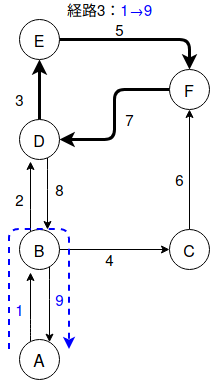
\includegraphics[height=6cm]{figure/second_route_T3.png}
            %\caption{}
            %\label{}
         \end{minipage}
         \begin{minipage}{0.50\hsize}
         \centering
         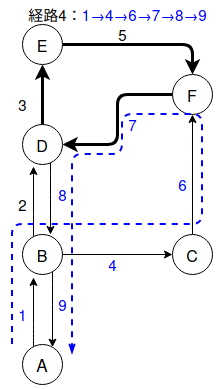
\includegraphics[height=6cm]{figure/second_route_T4.png}
            %\caption{}
            %\label{}
         \end{minipage}
      \end{tabular}
      \caption{Case 2の場合に残る故障候補とコマンド2に影響を受けるテレメトリが成す経路}%ここも変えたほうがいいかも
      \label{fig:sucond_route}  
\end{figure}

Case 2の結果になった時点で,コマンド2とテレメトリ3によって形成される経路3で確認できる故障候補
は存在しないので,経路4による検証を行うことになる.
経路4による検証結果は以下の図\ref{fig:TEL_result2}のように2通りが考えられる.
テレメトリ4が正常もしくは異常となる確率に関しては上述した式(\ref{eq:P_TEL_normal}),
(\ref{eq:P_TEL_abnormal})で求められ,以下の図のようになるため,
Case 2になる確率と合わせて考えると,Case 2-1またはCase 2-2になる確率は以下の式
(\ref{eq:T4=normal}),(\ref{eq:T4=abnormal})のように求まる.

\begin{figure}[H]
   \centering
      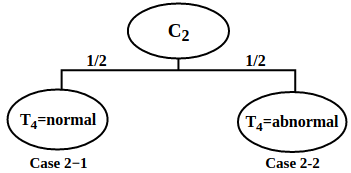
\includegraphics[height=3.5cm]{figure/TEL_result_process2.png}
      \caption{Case 2の時のコマンド2送信時の結果}
      \label{fig:TEL_result2}
\end{figure}
\vspace{-1zh}
\begin{eqnarray}
   P(\text{Case 2-1})  &=& P(\text{Case 2}) P(\text{T}_4=\text{normal}) \nonumber \\
     &=& \frac{7}{32} \times \frac{1}{2} = \frac{7}{64} \label{eq:T4=normal} \\
   P(\text{Case 2-2})  &=& P(\text{Case 2}) P(\text{T}_4=\text{abnormal}) \nonumber \\
     &=& \frac{7}{32} \times \frac{1}{2} = \frac{7}{64} \label{eq:T4=abnormal}
\end{eqnarray}

以上のような検証のプロセスを,
送信することで故障候補を切り分けられるコマンドが存在しなくなる,
もしくは故障箇所を特定するまで繰り返すことで,故障候補の切り分けを行う.
この流れをシステム上で先に計算し,人間がコマンドを送信する前に最終的に打つコマンドの総数を
見積もることが可能である.\\
以下の図\ref{fig:all_process}に,今回説明のために使用した例(図\ref{fig:all_process})%ここの参照がずれている
における検証の全プロセスを示す.

\begin{figure}[H]
   \centering
      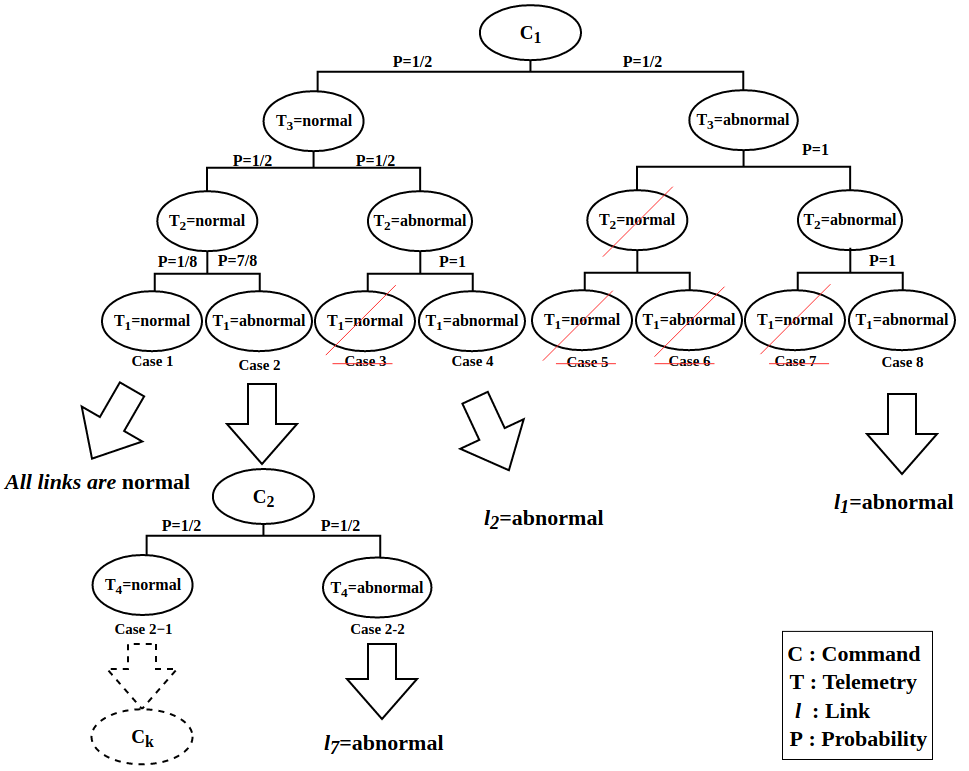
\includegraphics[height=10.0cm]{figure/all_process.png}
      \caption{検証プロセスの全体像}
      \label{fig:all_process}
\end{figure}
Case 1,4,8に関してはコマンド1を送信した時点で故障箇所の特定もしくは故障候補の棄却ができている
ので,その時点で検証は終了する.よって,検証にかかるコマンドの総数は1である.
一方で,Case 2の場合は,Case 2-1, 2-2へと続くため,コマンドの総数が2以上となる.
Case 2-2では故障箇所がリンク7であると特定できたためコマンドの総数は2となる.また,
Case 2-1では故障候補をリンク3もしくは5に絞り込むことができたが,故障箇所の特定までは至っていない.
そのため,残りの故障候補を確認できるコマンドを衛星システムが持つ場合には,次のコマンドを打つプロセス
の結果によってコマンドの総数が変わる.\\
ここでは簡単のため衛星システムがコマンド1と2のみを持つ場合を考え,コマンドの総数の期待値を算出
する.
以上で各Caseになる確率は算出しているので,それを用いると検証を行う際にコマンド1から選択した場合
のコマンドの総数は以下の式(\ref{eq:N Ck})のようになる.ここで,$\mathbb{C}$は検証が終了した
検証結果の集合であり,今回の例では$\mathbb{C} = \{\text{Case 1,Case 2-1, Case 2-2, Case 4, Case 8}\}$
である.

%これあっているのか不安になってきた.計算を見直す
\begin{eqnarray}
   N(\text{C}_1) &=& \sum_{\text{Case }i\in\mathbb{C}} P(\text{Case }i) N_{\text{Case }i} \nonumber \\
     &=& \frac{1}{32}\times 1 + \frac{7}{64}\times 2 + \frac{7}{64}\times 2 + \frac{1}{4}\times 1 +
     \frac{1}{2}\times 1 \nonumber \\
     &=& 1 \label{eq:N Ck}
\end{eqnarray}

同様にして,コマンド2から選択した場合も考えると,以下のように求まる.
\begin{eqnarray}
   N(\text{C}_2)  &=& 1.875 %途中式はipadにあるけどこれをちゃんと書くには図が必要になりそう..
\end{eqnarray}

このように,ある故障候補が残っている時に選択するコマンドの順番によって
コマンドの総数の期待値が変化する.
この期待値を「検証コマンド総数」と定義し,上述した指標と合わせて提示することで,どのコマンドから検証を開始することによって
少ないコマンド数で検証を終えることが可能なのかを人間が直感的に認識することが可能になる.
また検証プロセスにおいて,前検証結果に応じて検証コマンド総数は更新され,コマンド選択を行う際に
どのコマンドを選択すれば最終的に早く検証を終えることができるのかを示すことができる.\\
ここで,以上で示したコマンドの故障候補切り分け能力を示す指標を以下に再掲する.
\begin{itemize}
   \item 平均確認可能性及び確認可能リンク数
   \item 検証コマンド総数
\end{itemize}
%まあこれは故障状態によると思うから適切ではないか.

以上では簡単のため,各リンクの正常確率は全て0.5として統一していたが,
この情報は事前にモデルに組み込むことが可能であるため,実際の衛星に適した正常確率を考える
ことで,より効率的に故障個所の特定ができると考えられる.
%ここの説明微妙すぎるから修正
例えば,衛星の主要通信ラインである受信機と地上局間のリンクや,OBC間の
リンクは信頼性が高いと考え,正常確率を高く設定したり,
新規実装項目に関しては信頼性が低いと考え,低い正常確率
を設定したりするなどが挙げられる.


\begin{comment}
   
このことを踏まえて,あるコマンドとテレメトリのペアによって形成される経路(R)を通る情報によって
故障候補の確認を行う際,経路内に含まれる故障候補の数($N_F$とする)と
確認できるリンクの数の期待値($E$(R))の割合が,その経路を作るコマンドとテレメトリのペアが,
経路内の故障候補の内どれだけ確認することができるかを示している.\\
故障可能性リンクが多く含まれた,不確定性の大きな経路を通ると,

上で述べたように,切り分けを行っていくためには確実性が重要である.%???
そのため,その経路の「正の効果」を示す指標の一つとして確実性($C$(R)とする)を以下のように定義する.
\begin{eqnarray}
   C(\text{R})  &=& \frac{E(\text{R})}{N_F}
\end{eqnarray}
%ここらへん実装まで終わらして,ちゃんと有効であることを示せないと伝わらなさそう.
%有効でなければやり直しやが..

以上では,コマンドとそれによって影響を受けるテレメトリとのペアによって形成される経路に対して
「正の効果」を定義していたが,各コマンドが影響を与えるテレメトリは複数存在することが多くある.
人間が選択する際にはコマンドに対して指標が必要である.\\
あるコマンドに関連する経路が複数ある場合,それらに関する「確認可能リンク数」及び「確実性」
の単純和を取るだけでは対象としているリンクに被りが生じるため,コマンドの効果を表している
とは言えない.
そこで,各経路で被りが生じているリンクに関しては,
そのリンクを通る経路の中で距離が最短な経路が確認を行うものとし上の指標を再定義を行う.
あるコマンド(C$_k$とする)が影響を与える各テレメトリと成す経路の集合を
$\mathbb{R}_k = \{ \text{R}_{1}, \cdots ,\text{R}_{N_k} \}$(ただし$N_k$はコマンドC$_k$
によって形成される経路の数)とする.
%これは実装で必要になるかも
%また$\mathbb{R}_k$は経路長さの昇順でソートされている
また,各経路(R)$_{i}$に含まれる故障候補
の集合$\mathbb{F}_{i}$の直和を取り%少し間違っているから修正
$\mathbb{R}_k$に含まれる故障候補の集合を,
%なんかいい方法思いつかんから保留
\begin{eqnarray}
    \mathbf{F_k} &=& \sum_{i=1}^{N_k} \mathbb{F}_i
%    \bigcup_{i=1}^N \left( \bigcup_{i=1}^N \mathbb{F}_i - \bigcap_{i=1}^N\right) 
\end{eqnarray}
とし,$\mathbf{F_k}$に含まれるリンクの数を$\mathbf{N_{F_k}}$とする.
この時,C$_k$の「確認可能リンク数」及び「確実性」は以下のようになる.
\begin{eqnarray}
   E(\text{C}_k)  &=&\sum_{i\in \mathbf{F_k}} \prod_{j\in \mathbf{F_k}, j\neq i} P(l_i=\text{normal})  \\
   C(\text{C}_k)  &=& \frac{E(\text{C}_k)}{\mathbf{N_{F_k}}}
\end{eqnarray}
\end{comment}

%ここに情報量を組み込むといいかも?めんどくさい

%ここ洗練させる
\subsection{評価指標の使い分け}
次に,地上試験と軌道上での運用とで上述した指標の使い分けに関して
説明する.
\begin{comment}
   
%エントロピー使うなら平均は取らない.
まず,コマンドを打つことによってどれだけの情報が得られるかという点から,
そのコマンドを打つことによる情報量を考えた.

その指標として,コマンドの能力を情報量(エントロピー)の定義から考えた.
無理にエントロピーを使うのは間違っている気がする.情報量という考え方が妥当ではないか?
確率分布になっていないことを考えると.

コマンド$j$による切り分けの効果の指標を以下に定義する.\\
コマンド$j$が確認できるリンクの集合を$\mathbb{L}_j$とする.
この時,集合に含まれるリンクは$l_i\in \mathbb{L}_j$とする.
また,
「$\mathbb{L}_j$を確認する」という事象を$\Omega$とすると,
各リンク$l_i$を確認するという事象$E_i \in \Omega$として,

ここで,各リンクの状態を確認する方法として,本手法ではコマンドによるアクセスのみを考えているので
「リンク$l_i$を確認する」という事象と,「リンク$l_i$を確認できるコマンドを選択する」
という事象の確率は等価である.%各コマンドを選ぶ確率は等しいという仮定が入っているような気がする.
よって,「リンク$l_i$を確認する」という事象の確率は式(\ref{eq:Pi})
で与えられる.この時,事象($E_i$)が起こった時に受け取る(選択)情報量$I_i$は式(\ref{eq:I_i})
で定義される.

\begin{eqnarray}
   P(E_i) &=& \frac{\text{Number of command which can verify Link }i}{\text{All command number}} \label{eq:Pi}\\
   I(E_i) &=& -\log{P_{i}} \label{eq:I_i} \\
\end{eqnarray}
確率$P(E_i)$は確率分布であるという説明が必要

よって事象$\Omega$による平均情報量は
\begin{eqnarray}
   H(P) &=& -\sum_{E_i \in \Omega} P(E_i)\log{P(E_i)} 
\end{eqnarray}
となる.定性的な意味としては,コマンドを打つことによってどれだけの情報
が得られる可能性があるかを示している.

コマンドが絞り込むことのできる能力という点はどうする?

以上の指標を踏まえた上でどのように提示し人間の判断を支援するのかを考える.
\end{comment}

%地上試験と運用時の両方で使い分けることのできるフレームワークであることを示す.
地上試験では,電源供給に関してはバッテリではなく安定化電源を用いた試験コンフィギュレーションで
行うことが多い.そのため,上述した電力の制約に関しては地上試験で考慮する必要はない.
また,試験時は衛星を試験台に固定して行うため,姿勢変化に関する制約も考慮する必要は
ない.
これらを踏まえると,地上試験で安全を重視して二次故障などを引き起こさないように
切り分けを行うためには,波及効果の大きさを示す指標である
「コマンドを打つことで変化するテレメトリの数」が小さなコマンドを選択すれば良い.\\
また,地上試験では衛星全体ではなく部分的なコンポーネントを組み上げた状態による試験も多数行う.
システムを構成するコンポーネントの種類によっては,コマンドによって引き起こされる状態変化
の波及効果によって二次故障が発生する可能性は低い場合も考えられる.
そのような際には,コマンドの故障候補切り分け能力
を重視し,「平均確認可能性」及び「確認可能リンク数」が高く,
「検証コマンド総数」が小さいコマンドを選択することで効率的な切り分けが行える.

%もう少し軌道上での具体例があると説得力が増すかもしれない.
%クリティカルイベントの際に役立つとか
運用中は上述した電力や姿勢に関する制約を考える必要がある.また,
可視時間中に不具合原因の特定を行わなければならないなどの
時間制約の厳しい条件下での分析が必要になることもある.
そのような時には,リスクを大きく取りつつ効果の大きなコマンドを選択する必要がある.
一般に,故障候補を切り分ける能力が高いコマンドは,「コマンドを打つことで変化するテレメトリの数」
も大きくなる.
よって,運用時は上で示した全ての指標を元に,コマンドによって二次故障などが
発生するリスクと,故障候補切り分けの効率のトレードオフを考慮し
コマンドの選択を行う必要がある.


\expandafter\ifx\csname ifdraft\endcsname\relax
  \end{document}
\fi